\newpage
\section*{Zielsetzung}
Aufnehmen und analysieren von dem Emissionsspektrum einer CU-
Röntgenröhre und verschiedener Absorbtionsspektren.
\section{Theorie}
\subsection{Erzeugung Röntgenstrahlung}
Innerhalb einer evakuierten Röhre werden Elektronen aus einer Glühkathode
auf eine Anode hin beschleunigt.\\
\\Die Röntgenstrahlung ist auf zwei Effekt zurückzuführen.

\subsubsection*{Bremsstrahlung}
Durch Abbremsen der freien Elektronen in einem Elektrischen Feld 
wird Energie durch Röntgenquanten frei. Die Energie entspricht dabei
dem Energieverlust der Abbremsung. Bei vollständiger Abbremsung ergibt
sich die Wellenlänge
\begin{equation}
    \lambda_{min}=\frac{h \cdot c}{e_0U}.
    \label{eqn:minW}
\end{equation}
Da hierbei verschieden hohe kinetische Energien abgegeben werden können,
äußert siche die Bremsstrahlung im Spektrum durch einen Kontinuierlichen
Verlauf.
\begin{figure}
    \centering
    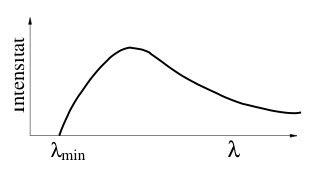
\includegraphics[width=0.4\textwidth]{plots/wellenberg.jpg}
    \caption{Dargstellt ist das Bremsspektrum. Die kleinsten Wellenlängen $\lambda$
    entspricht dabei den Elektronen der größten Energien.\cite[1]{anleitung}}
\end{figure}

\subsubsection*{Charakteristisches Spektrum}
Beim Auftreffen der Elektronen auf das Anodenmaterial wird dieses ionisiert, sodass
ein gebundenes Elektron von einer höheren Schale auf eine niedrigere Schale fallen kann und dabei
Energie in Form von Röntgenquanten emitiert. Die abgestrahlte Energie entspricht dann der Differenz
der Energieniveaus.
\begin{equation}
    h\cdot v=E_m-E_n
    \label{eqn:energii}
\end{equation}
Das charakteristische Spektrum ist vom Anodenmaterial abhängig und zeichnet sich im
Röntgenspektrum durch scharfen Linien aus.
Die frei werdende Energie hängt dabei von den Schalen ab aus der das Elektron herausgelöst
und aus der das neue Elektron hinabsteigt ab. Die Schalenenergien werden über den Index $m$ und $n$
unterschieden. Der Prozess kann zwischen verschiedenen Schalen (genannt: K,L,M) im Atom 
stattfinden. Die Großbuchstaben verwendet man dabei, um die Position des herausgelösten Elektrons zu 
beschreibten, während die griechischen Indizes die Schale beschreiben aus der das neue Elektron 
nachrutscht.
Die Energie eines Elektronensprungs ergibt sich somit mit Gl. \ref{eqn:energii}
\begin{equation}
    E_n=-R_{\infty}\cdot z_{\text{eff}}^2 \cdot \frac{1}{n^2},
    \label{eqn:energiii}
\end{equation}
wobei die Rydbergenergie $R_{\infty}=13.6$eV und die effektive Kernladung 
$z_{eff}=z-\sigma$ mit der Abschirmkonstante $\sigma$ ist. Dabei wird berücksichtigt,
dass die Hüllenelektronen die Coulomb Anziehung auf das äußere Elektron abschirmen.
\begin{figure}
    \centering
    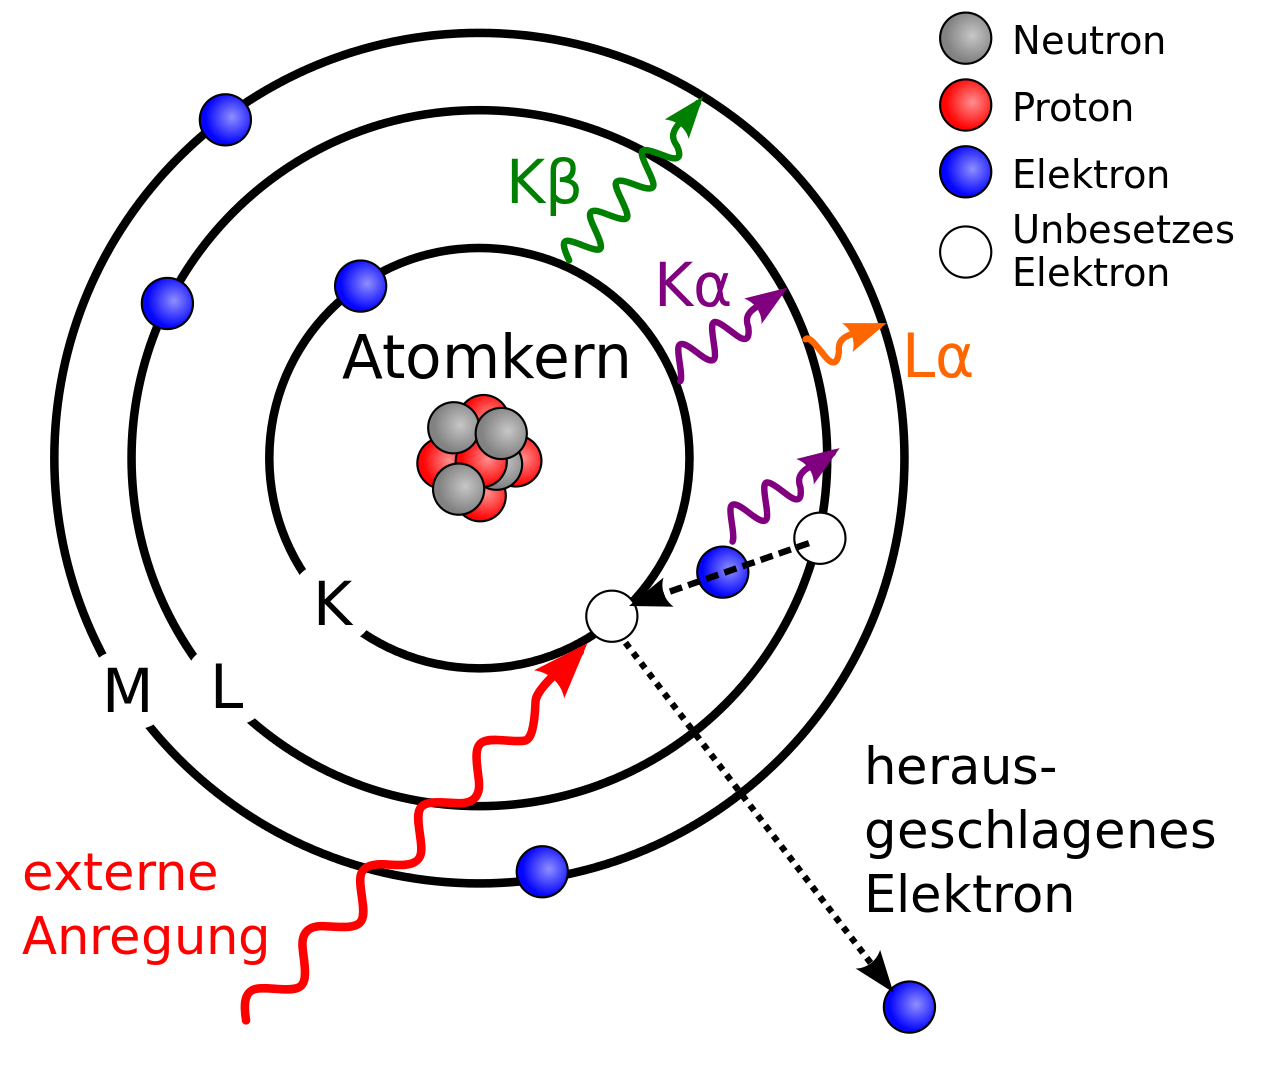
\includegraphics[width=0.4\textwidth]{plots/chS.png}
    \caption{Darstellung des Prozesses der Röntenemission durch die
    Ionisation des Atoms. Das (Röntgen)Photon wirkt als exteren Anregung, welches
    ein Elektron aus der inneren Schale schlägt. Ein anderes Elektron aus einer
    höheren Schale rutscht nach und gibt Energie in Form von Strahlung ab.\cite{wiki}}
\end{figure}
Für die Energie einer Überganslinie aus der Abschirmkonstante $\sigma$ der einzelenen Elektronen, der Energieniveaus
der Schalen und der Kernladnungszahl $Z$ ergibt sich mit Gl. \ref{eqn:energiii} in Gl. \ref{eqn:energii}
\begin{equation}
    E_{\text{Schale}_{m,n}}=R_{\infty}\cdot (Z-\sigma_n)^2\cdot \frac{1}{n^2}-R_{\infty}\cdot (Z-\sigma_m)\cdot \frac{1}{m^2}
\end{equation}
\subsection{Bragg-Bedingung}
Die Energie der Strahlung kann mithilfe der Bragg-Reflexion ermittelt werden.
Durch Beugung an einem dreidimsensionalen Gitter (LiF-Kristall) mit der Gitterkonstante $d$ 
entsteht eine konstruktive Interferenz bei einem Braggwinkel $\Theta$. Durch die Bragg-Bedingung
\begin{equation}
    2 d \sin(\Theta)=n\lambda,
    \label{eqn:bragg}
\end{equation}
ergibt sich die Wellenlänge $\lambda$. n ist dabei die Beugungsordunung.
\begin{figure}
    \centering
    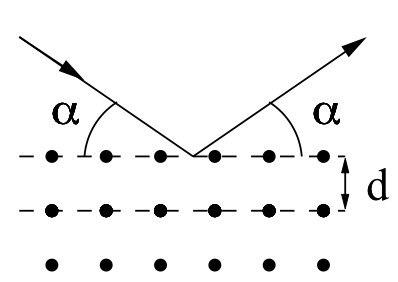
\includegraphics[width=0.3\textwidth]{plots/bragg.jpg}
    \caption{Darstellung der Bragg-Reflexion an einem Gitter mit der
    Gitterkonstante $d$ und dem Bragg-Winkel $\alpha$.\cite[3]{anleitung}}
\end{figure}


\subsection{Absorbtion}
Treffen Röntgenstrahlen auf ein Material, so nimmt dieses die Strahlung zum Teil
auf (Absorbtion). Diese ist zum Teil vom Material, derer Dicke $d$ und der Energie 
der Strahlung abhängig.
Die Absorbtion entsteht durch Auftretten von Effekten wie des Photo-Effekts und der
Compton-Streuung bei Energien $E<1\si{MeV}$, darüber hinaus sinkt der Wirkungsquerschnitt 
und weiter Effekte dominieren die Absorbtion.
\begin{equation}
    \frac{I(d)}{I_0}=e^{-\mu d}=:\tau
\end{equation}
Dabei ist $\mu$ der Absorbtionskoeffizient.\\
Dieser ist abhängig von der Energie der Strahlung und nimmt bei zunehmender
Strahlungsenergie ab. $\mu$ steigt allerdings sprunghaft an, wenn die Strahlungsenergie
gleich groß der Bindungsenergie eines Elektrons aus der nächsten inneren Schale ist.
Man spricht von einer Absorbtinskante.
\begin{figure}[H]
    \centering
    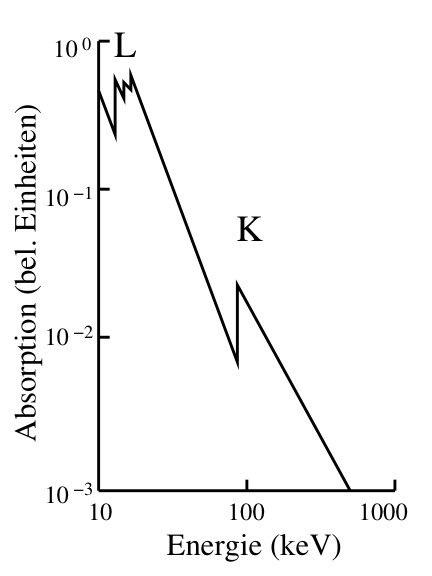
\includegraphics[width=0.25\textwidth]{plots/kante.jpg}
    \caption{Dargestellt ist ein Absorbtionspektrum, die Sprünge der Absorbtionskanten sind deutlich zu erkennen.\cite[2]{anleitung}}
\end{figure}
Um ein Elektron auf eine nächsthöhere Schale zu bringen benötigt es eine Strahlungsfrequenz
\begin{equation}
    h\cdot v_{\text{abs}}=E_n-E_{\infty}
\end{equation}
Da die Elektronen in einer Schale nicht alle die selbe potenzielle Energie
besitzen spalten sich die Hauptkanten auf in eng an einanerliegene Linien (Feinstrukturen),
diese werden im folgenden allerdings nicht weiter aufgelöst. Diese zugehörigen
Energien $E_{n,j}$ hängen nun neben dem Energieniveau $n$ und der effektiven Kernladungszahl
auch vom Spin $j$ des Elektrons auf der Schale ab.
Es gilt die Sommerfeldsche Feinstrukturformel
\begin{equation}
    E_{n,j}=-R_{\infty}\cdot \left(z_{\text{eff}}^2\cdot \frac{1}{n^2}+\alpha^2z_{\text{eff}}^4\cdot \frac{1}{n^3}\cdot \left(\frac{1}{j+\frac{1}{2}}-\frac{3}{4n}\right)\right).
\end{equation}
Für die K-Kante (n=1) ergibt sich nach der Sommerfledschen Feinstrukturformel
die Abschirmkonstante
\begin{equation}
    \sigma_K=Z-\sqrt{\frac{E_K}{R_{\infty}}-\frac{\alpha^2Z^4}{4}}
    \label{eqn:sigmaZ}
\end{equation}

So folgt für eine Abschätzung der Abschirmkonstanten $\sigma$ für Kupfer
mit $n=1$,$m=2$ und $l=3$,
\begin{align}
    \sigma_1 &= Z-\sqrt{\frac{E_{K,abs}}{R}},\\
    \sigma_2 &= Z-\sqrt{4\cdot (Z-\sigma_1)^2-\frac{4E_{K\alpha}}{R}}, \\
    \sigma_3 &= Z-\sqrt{9\cdot(Z-\sigma_1)^2-\frac{9E_{K\beta}}{R}} .
    \label{eqn:sigma}
\end{align}

\subsection{Mosley'sch Gesetz}
Nach 
\begin{equation}
    E_K=Rh(z-\sigma)^2
    \label{eqn:mos}
\end{equation}
ist die Energie der $K_{\alpha}$-Strahung proprtional zu $z^2$ bei $n=1$.

\subsection{Halbwertsbreite (Full Width at Half Maximum)}
Die Breite bie halber Höhe (kurz: FWHM) beschreibt "die Differenz zwischen 
den beiden Argumentwerten, für die die Funktionswerte auf die 
Hälfte des Maximums abgesunken sind."\cite{wiki2}
\begin{figure}[H]
    \centering
    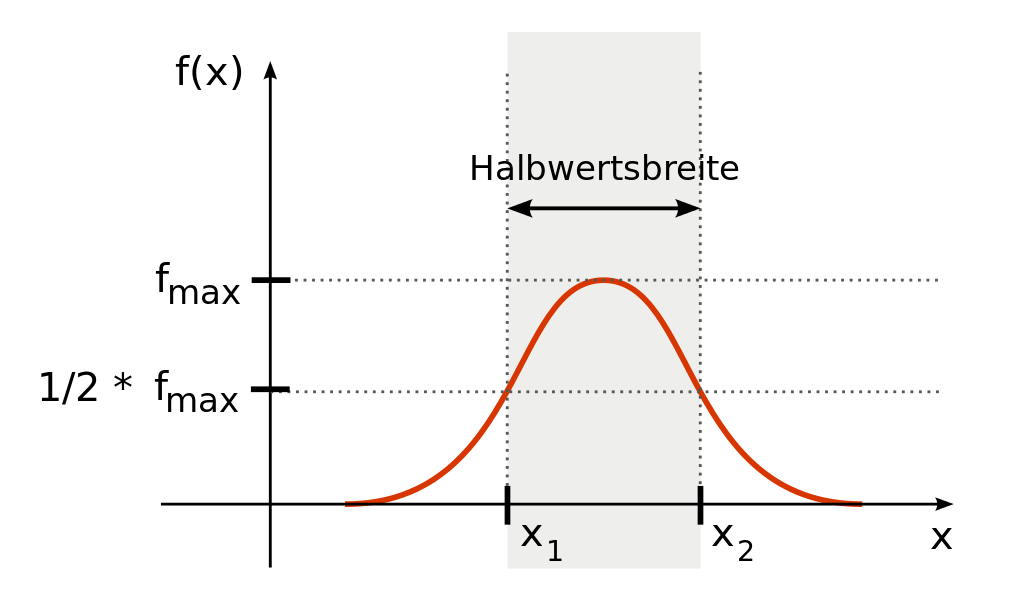
\includegraphics[width=0.4\textwidth]{plots/Halbwertsbreite.png}
    \caption{Darstellung der Halbwertsbreite.\cite{wiki2}}
\end{figure}
\label{subsec:halbwert}

